% "{'classe':('PSI'),'chapitre':'dyn_pfd_co','type':('application'),'titre':'Chargement et déchargement des cargos porte-conteneurs', 'source':'Centrale Supélec PSI 2013','comp':('C1-05','C2-09'),'corrige':True}"
%\setchapterimage{bandeau}
\chapter*{Application \arabic{cptApplication} \\ 
Chargement et déchargement des cargos porte-conteneurs  \ifnormal $\star$ \else \fi \ifdifficile $\star\star$ \else \fi \iftdifficile $\star\star\star$ \else \fi
-- \ifprof Corrigé \else Sujet \fi}
\addcontentsline{toc}{section}{Application \arabic{cptApplication} : 
Chargement et déchargement des cargos porte-conteneurs  \ifnormal $\star$ \else \fi \ifdifficile $\star\star$ \else \fi \iftdifficile $\star\star\star$ \else \fi
-- \ifprof Corrigé \else Sujet \fi}

\iflivret \stepcounter{cptApplication} \else
\ifprof  \stepcounter{cptApplication} \else \fi
\fi

\setcounter{question}{0}
\marginnote{Centrale Supélec PSI 2013.}
\marginnote[1cm]{
\UPSTIcompetence[2]{C1-05}
\UPSTIcompetence[2]{C2-09}
}
\begin{marginfigure}
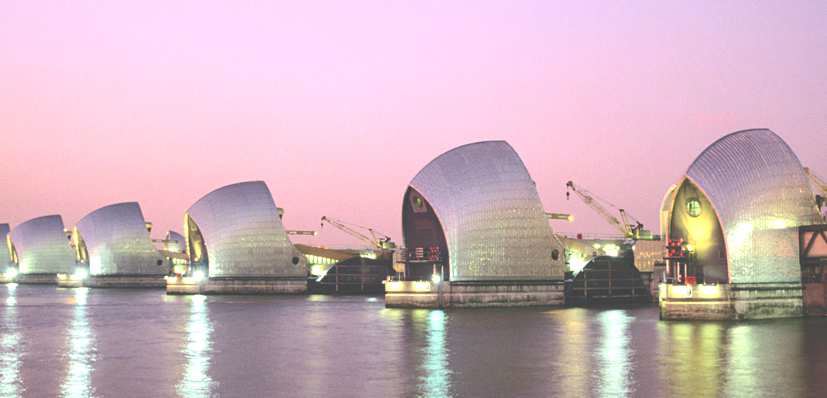
\includegraphics[width=\linewidth]{fig_00}
\end{marginfigure}


\subsection*{Modélisation dynamique du comportement de la charge}

\begin{obj}
Déterminer les équations du mouvement du conteneur de façon à en obtenir un modèle simple pour
la synthèse de la commande.
\end{obj}

\ifprof
\else
En vue d’élaborer une commande automatisée du déchargement des conteneurs, une bonne compréhension de
la dynamique du système est nécessaire. Cette partie vise à établir les équations du mouvement du conteneur.
%Seul le vérin 3 est libéré. 
La charge peut alors balancer selon le modèle présenté ci-après. Dans cette étude, la vitesse de vent nulle. On fait l'hypothèse que le conteneur est suspendu à un seul câble indéformable, en liaison pivot à ses extrémités. Les liaisons entre les solides 0, 1, 2 et 3 sont supposées parfaites.
Le portique support du chariot est noté 0, le chariot 1, le câble 2 et l’ensemble \{spreader + conteneur\} 3.

\paragraph*{Paramétrage}
\begin{itemize}
\item Le repère $\mathcal{R}_0=\repere{O_0}{x_0}{y_0}{z_0}$ est lié au portique fixe ; il est supposé
galiléen avec $\vect{z_0}$ l’axe vertical ascendant.
\item La position du chariot telle que $\vect{OE} = y_{ch}(t) \vect{y_0}$ est notée $y_{ch}(t)$ ;
l’angle $\angl{z_0}{z_2}$ d’inclinaison du câble $\theta(t)$ et l’angle $\angl{z_2}{z_3}$ d’inclinaison
du conteneur par rapport au câble  $\beta(t)$.
\end{itemize}

\begin{marginfigure}
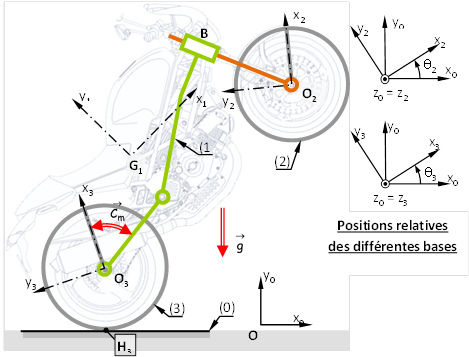
\includegraphics[width=\linewidth]{fig_01}
\end{marginfigure}

\paragraph*{Données}
\begin{itemize}
\item $\mathcal{R}_1=\repere{E}{x_0}{y_0}{z_0}$  repère lié au chariot de levage 1.
\item $\mathcal{R}_2=\repere{E}{x_0}{y_2}{z_2}$  repère lié au câble 2; $\ell_2 = \SI{50}{m}$ la longueur $EF$
du câble ; la masse est négligée.
\item $\mathcal{R}_3=\repere{F}{x_0}{y_3}{z_3}$  repère lié à l’ensemble \{spreader + conteneur\};
$m_3 = \SI{50}{tonnes}$ la masse du solide 3 ; $G_3$ le centre de gravité du
solide 3, tel que $\vect{G_3F}=h_3\vect{z_3}$ où $h_3 = \SI{2,5}{m}$; la matrice d’inertie du solide 3 s’écrit
$\inertie{3}{G_3}=\matinertie{A_3}{B_3}{C_3}{0}{0}{0}{\left(\vect{x_0},\vect{y_3},\vect{z_3} \right)}$ où $\left| \begin{array}{l} A_3 = \SI{52e3}{kg.m^2} \\ B_3 = \SI{600e3}{kg.m^2} \\ C_3 = \SI{600e3}{kg.m^2} \end{array}\right.$. 
\item la motorisation $M_D$ du mouvement de direction exerce, par l’intermédiaire de câbles, des actions mécaniques sur (1) qui se réduisent
à un glisseur de la forme $\vectf{M_D}{1} =F \vect{y_0}$ ;
\item l’action mécanique du câble sur le spreader est notée $\vectf{2}{3} =F_{23} \vect{z_2}$.
\end{itemize}




\fi

\question{Après avoir réalisé le graphe de structure, déterminer le nombre de degrés de liberté et le nombre d’actionneurs du modèle proposé figure précédente. En
déduire le nombre de degrés de liberté non motorisés. Expliquer pourquoi il est difficile de poser le conteneur
sur un camion avec précision ?}
\ifprof

\begin{marginfigure}
\centering
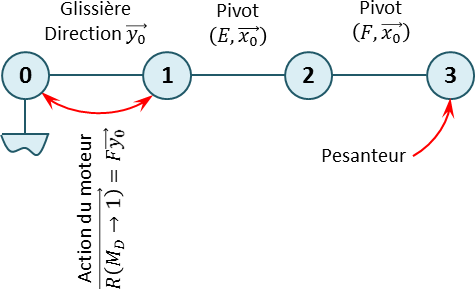
\includegraphics[width=\linewidth]{cor_01}
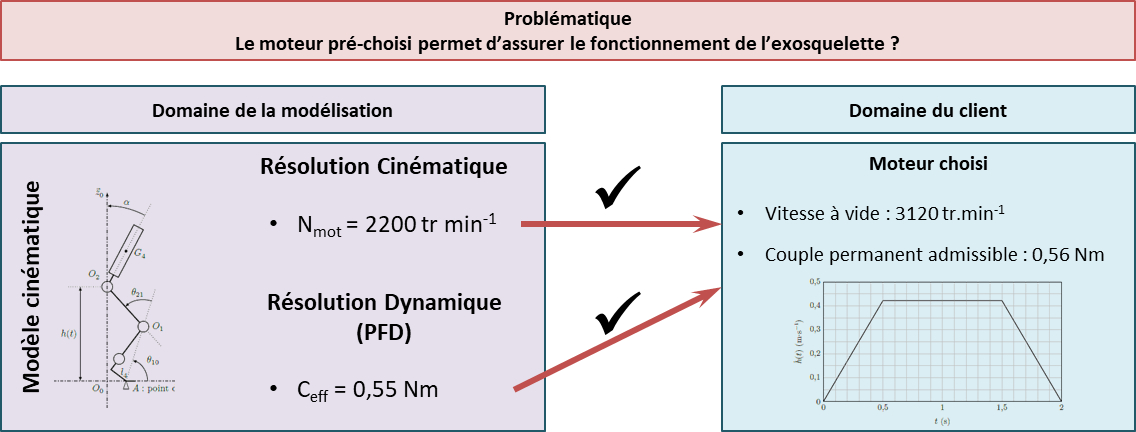
\includegraphics[width=.8\linewidth]{cor_02}
\end{marginfigure}

\begin{corrige} ~\\

Le système a trois mobilités : 
\begin{itemize}
\item la translation de la liaison glissière de longueur $y_{ch}(t)$ (degré de liberté motorisé);
\item la rotation du câble d'angle $\theta(t)$ (degré de liberté non motorisé);
\item la rotation du conteneur d'angle $\beta(t)$ (degré de liberté non motorisé). 
\end{itemize}

Les deux liaisons pivot n'étant pas freinées ou motorisées, lorsque le chariot se positionne au-dessus du camion le conteneur va se balancer, ce qui rend difficile la dépose du conteneur. 

\end{corrige}
\else
\fi

\question{Déterminer littéralement, au point $G_3$, la vitesse $\vectv{G_3}{3}{0}$ puis le torseur dynamique $\torseurdyn{3}{0}$ de l’ensemble \{conteneur + spreader\} (3) dans son mouvement par rapport au repère galiléen $\mathcal{R}_0$.}
\ifprof
\begin{corrige}
$\vectv{G_3}{3}{0}=   \left[\dfrac{\dd \vect{OG_3}}{\dd t}\right]_{\rep{0}}=   \left[\dfrac{\dd }{\dd t}\left(
\vect{OE}+\vect{EF}+\vect{FG_3} \right)\right]_{\rep{0}}$ 
$=   \left[\dfrac{\dd }{\dd t}\left(
y_{ch}(t) \vect{y_0}-\ell_2\vect{z_2}-h_3\vect{z_3} \right)\right]_{\rep{0}}$. 

On a : 
\begin{itemize}
\item $ \left[\dfrac{\dd \vect{z_2}}{\dd t}\right]_{\rep{0}}=\left[\dfrac{\dd \vect{z_2}}{\dd t}\right]_{\rep{2}}+\vecto{2}{0} \wedge \vect{z_2}=\dot{\theta} \vect{x_2}\wedge \vect{z_2}=-\dot{\theta} \vect{y_2}$;
\item $ \left[\dfrac{\dd \vect{z_3}}{\dd t}\right]_{\rep{0}}=\left[\dfrac{\dd \vect{z_3}}{\dd t}\right]_{\rep{3}}+\vecto{3}{0} \wedge \vect{z_3}=\left(\dot{\theta}+\dot{\beta}\right) \vect{x_2}\wedge \vect{z_3}=-\left(\dot{\theta}+\dot{\beta}\right) \vect{y_3}$;
\item $ \left[\dfrac{\dd \vect{y_2}}{\dd t}\right]_{\rep{0}}=\dot{\theta} \vect{z_2}$;
\item $ \left[\dfrac{\dd \vect{y_3}}{\dd t}\right]_{\rep{0}}=\left(\dot{\theta}+\dot{\beta}\right) \vect{z_3}$.
\end{itemize}

$\vectv{G_3}{3}{0}=   
\dot{y}_{ch}(t) \vect{y_0}+\ell_2\dot{\theta} \vect{y_2}+h_3\left(\dot{\theta}+\dot{\beta}\right) \vect{y_3}$.

$\vectg{G_3}{3}{0}=   
\ddot{y}_{ch}(t) \vect{y_0}+\ell_2\ddot{\theta} \vect{y_2}+h_3\left(\ddot{\theta}+\ddot{\beta}\right) \vect{y_3}
+   
\ell_2\dot{\theta}^2 \vect{z_2}  +h_3\left(\dot{\theta}+\dot{\beta}\right)^2\vect{z_3} $.

Par ailleurs, $G_3$ étant le centre d'inertie, de 3, on a $\vectmd{G_3}{3}{0}=\left[\dfrac{\dd \vectmc{G_3}{3}{0}}{\dd t}\right]_{\rep{0}}=\left[\dfrac{\dd A_3 \left(\dot{\theta}+\dot{\beta} \right)\vect{x_0}}{\dd t}\right]_{\rep{0}}=A_3 \left(\ddot{\theta}+\ddot{\beta} \right)\vect{x_0}$.

On a donc, $\torseurdyn{3}{0}=\torseurl{M_3\left(\ddot{y}_{ch}(t) \vect{y_0}+\ell_2\ddot{\theta} \vect{y_2}+h_3\left(\ddot{\theta}+\ddot{\beta}\right) \vect{y_3}
+   
\ell_2\dot{\theta}^2 \vect{z_2}  +h_3\left(\dot{\theta}+\dot{\beta}\right)^2\vect{z_3}\right)}{A_3 \left(\ddot{\theta}+\ddot{\beta} \right)\vect{x_0}}{G_3}$
\end{corrige}
\else
\fi

\question{En précisant l’isolement et le bilan des actions mécaniques extérieures, déterminer l’équation différentielle
de résultante reliant les paramètres $\theta(t)$, $\beta(t)$%$\beta(t)$
 et $y_{ch}(t)$, sans inconnue de liaison et sans l'action du moteur.}
\ifprof
\begin{corrige}

D'une part, on peut se dire qu'on va utiliser le résultat de la question précédente. D'autre part, le sujet demande une équation de résultante sans aucune action mécanique. Si on isole le solide 3, il va donc falloir projeter sur une direction ne faisant pas intervenir d'action mécanique. Les données précisent que l'action du câble est suivant $\vect{z_2}$, on peut donc suggérer de réaliser le thorème de la résultante dynamique appliqué au solide 3 en projection sur $\vect{y_2}$. 

Le bilan des actions mécaniques est donc le suivant : 
\begin{itemize}
\item action de la pesanteur sur 3;
\item action de 2 sur 3.
\end{itemize}

On a donc :
$-M_3 g \vect{z_0}\cdot \vect{y_2} = 
\left( M_3\left(\ddot{y}_{ch}(t) \vect{y_0}+\ell_2\ddot{\theta} \vect{y_2}+h_3\left(\ddot{\theta}+\ddot{\beta}\right) \vect{y_3}
+   
\ell_2\dot{\theta}^2 \vect{z_2}  +h_3\left(\dot{\theta}+\dot{\beta}\right)^2\vect{z_3}\right)\right) \cdot \vect{y_2}$

$ \Leftrightarrow -M_3 g \sin \theta  = 
 M_3\left(\ddot{y}_{ch}(t) \cos \theta +\ell_2\ddot{\theta} +h_3\left(\ddot{\theta}+\ddot{\beta}\right)\cos \beta 
-h_3\left(\dot{\theta}+\dot{\beta}\right)^2\sin\beta \right)$


\vspace{.6cm}
Résolution faisant intervenir $F$ -- Non demandé.

L'équation de résultante étant demandée, on peut aussi isoler une pièce (ou un ensemble de pièces) en translation rectiligne. On isole donc \textbf{(1+2+3)} et on réalise un théorème de la résultante dynamique en projection sur $\vect{y_0}$. 

Bilan des actions mécaniques : 
\begin{itemize}
\item action de la pesanteur sur 3 (la résultante n'a pas de composante sur $\vect{y_0}$);
\item action de la pesanteur sur 1 (négligée) (la résultante n'a pas de composante sur $\vect{y_0}$);
\item action de 0 sur 3 (glissière) (la résultante n'a pas de composante sur $\vect{y_0}$);
\item action du moteur sur 1.
\end{itemize}

On applique le TRD sur $\vect{y_0}$ :
$F = \vectrd{1+2+3}{0}\cdot \vect{y_0}= \underbrace{\vectrd{1}{0} \cdot  \vect{y_0}}_{=0 \text{(masse négligée)}}+ \underbrace{\vectrd{2}{0}\cdot  \vect{y_0}}_{=0 \text{(masse négligée)}} + \vectrd{3}{0}\cdot \vect{y_0}$

 $ \Rightarrow F = \left( M_3\left(\ddot{y}_{ch}(t) \vect{y_0}+\ell_2\ddot{\theta} \vect{y_2}+h_3\left(\ddot{\theta}+\ddot{\beta}\right) \vect{y_3}
+   
\ell_2\dot{\theta}^2 \vect{z_2}  +h_3\left(\dot{\theta}+\dot{\beta}\right)^2\vect{z_3}\right)\right) \cdot \vect{y_0}$

 $ \Leftrightarrow F =  M_3\left(\ddot{y}_{ch}(t) +\ell_2\ddot{\theta} \cos \theta +h_3\left(\ddot{\theta}+\ddot{\beta}\right) \cos \left( \beta+\theta\right)
-
\ell_2\dot{\theta}^2 \sin \theta   -h_3\left(\dot{\theta}+\dot{\beta}\right)^2  \sin \left( \beta+\theta\right)\right) $
\end{corrige}
\else
\fi

\question{En précisant l’isolement et le bilan des actions mécaniques extérieures, déterminer les équations différentielles
reliant les paramètres $\theta(t)$, $\beta(t)$  et $y_{ch}(t)$ et sans inconnue de liaison. La méthode sera clairement séparée des calculs.}
\ifprof
\begin{corrige}
Le TRD appliqué à 3 en projection suivant $\vect{z_2}$ se traduit par : 

$F-M_3 g \vect{z_0}\cdot \vect{z_2} = 
\left( M_3\left(\ddot{y}_{ch}(t) \vect{y_0}+\ell_2\ddot{\theta} \vect{y_2}+h_3\left(\ddot{\theta}+\ddot{\beta}\right) \vect{y_3}
+   
\ell_2\dot{\theta}^2 \vect{z_2}  +h_3\left(\dot{\theta}+\dot{\beta}\right)^2\vect{z_3}\right)\right) \cdot \vect{z_2}$

$\Leftrightarrow F-M_3 g \cos \theta  = 
 M_3\left(- \ddot{y}_{ch}(t) \sin \theta +h_3\left(\ddot{\theta}+\ddot{\beta}\right) \sin\beta
+   
\ell_2\dot{\theta}^2   +h_3\left(\dot{\theta}+\dot{\beta}\right)^2\cos \beta \right) $.



Le TMD appliqué à 3 au point $F$ en projection suivant $\vect{x_0}$ se traduit par : 

$\vect{FG_3}\wedge \left(-M_3g \vect{z_0} \right) \cdot \vect{x_0} =\left(\vectmd{G_3}{3}{0}+\vect{FG_3}\wedge \vectrd{3}{0}\right)\cdot \vect{x_0}$

$\Leftrightarrow -h_3 \vect{z_3} \wedge \left(-M_3g \vect{z_0} \right) \cdot \vect{x_0} =A_3 \left(\ddot{\theta}+\ddot{\beta} \right)$

$\Leftrightarrow - M_3gh_3 \sin\left( \beta + \theta\right) =A_3 \left(\ddot{\theta}+\ddot{\beta} \right)$.
\end{corrige}
\else
\fi


\question{En supposant que $\theta$, $\beta$, $\dot{\theta}$ et $\dot{\beta}$ sont petits, linéariser les équations précédentes.}
\ifprof
\begin{corrige}
\begin{itemize}
\item On a 
$ -M_3 g \sin \theta  = 
 M_3\left(\ddot{y}_{ch}(t) \cos \theta +\ell_2\ddot{\theta} +h_3\left(\ddot{\theta}+\ddot{\beta}\right)\cos \beta 
-h_3\left(\dot{\theta}+\dot{\beta}\right)^2\sin\beta \right)$. En linéarisant, on obtient 
$ -M_3 g \theta  = 
 M_3\left(\ddot{y}_{ch}(t) +\ell_2\ddot{\theta} +h_3\left(\ddot{\theta}+\ddot{\beta}\right) 
-h_3\left(\dot{\theta}+\dot{\beta}\right)^2\beta \right)$. En considérant que $\dot{\theta}$ et $\dot{\beta}$ sont petits, on a : 
$ -M_3 g \theta  = 
 M_3\left(\ddot{y}_{ch}(t) +\ell_2\ddot{\theta} +h_3\left(\ddot{\theta}+\ddot{\beta}\right)  \right)$.
\item  On a : $F-M_3 g \cos \theta  = 
 M_3\left(- \ddot{y}_{ch}(t) \sin \theta +h_3\left(\ddot{\theta}+\ddot{\beta}\right) \sin\beta
+   
\ell_2\dot{\theta}^2   +h_3\left(\dot{\theta}+\dot{\beta}\right)^2\cos \beta \right) $. En linéarisant, on obtient :
$F-M_3 g  = 
 M_3\left(- \ddot{y}_{ch}(t) \theta +h_3\left(\ddot{\theta}+\ddot{\beta}\right) \beta
+   
\ell_2\dot{\theta}^2   +h_3\left(\dot{\theta}+\dot{\beta}\right)^2 \right) $
En considérant que $\dot{\theta}$ et $\dot{\beta}$ sont petits, on a : 
$F-M_3 g  = 
 M_3\left(- \ddot{y}_{ch}(t) \theta +h_3\left(\ddot{\theta}+\ddot{\beta}\right) \beta
 \right) $.
 \item On a : $ M_3gh_3 \sin\left( \beta + \theta\right) =A_3 \left(\ddot{\theta}+\ddot{\beta} \right)$ En linéarisant, on obtient  $M_3gh_3 \left( \beta + \theta\right) =A_3 \left(\ddot{\theta}+\ddot{\beta} \right)$.
 \end{itemize}

\end{corrige}
\else
\fi


Les courbes temporelles ont été obtenues par simulation, à partir des équations précédentes, pour un
échelon en $y_{ch}(t)$ de $\SI{10}{m}$. 

\ifprof
\begin{multicols}{2}
\begin{center}
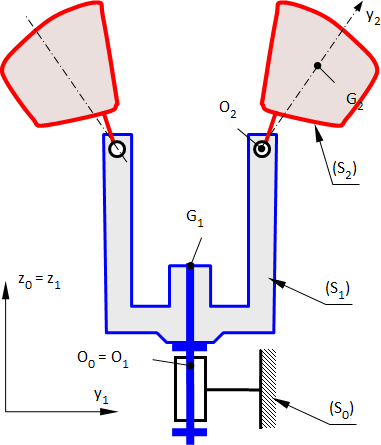
\includegraphics[width=.8\linewidth]{fig_02}
\end{center}

\begin{center}
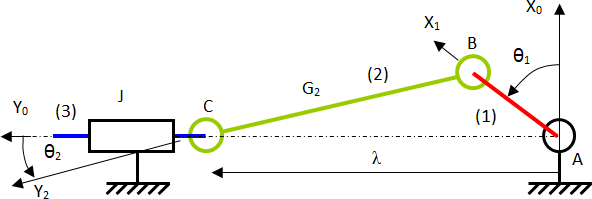
\includegraphics[width=.8\linewidth]{fig_03}
\end{center}
\end{multicols}
\else
\begin{marginfigure}[-7cm]
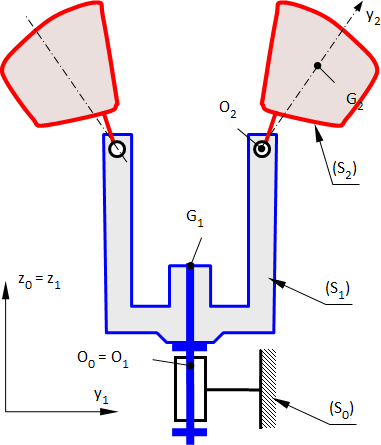
\includegraphics[width=\linewidth]{fig_02}
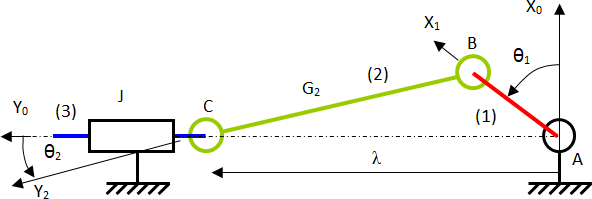
\includegraphics[width=\linewidth]{fig_03}
\end{marginfigure}

\fi


\ifprof
\else
\begin{marginfigure}
\centering

\includegraphics[width=3cm]{Cy_04_03_PFD_CO_App_04_ChargementCargo_qr}
\end{marginfigure}
\fi

\question{Proposer une simplification de la modélisation précédente.   }
\ifprof
\begin{corrige}
L'amplitude des oscillations de $\beta$ est 10 fois inférieure aux oscillations de $\theta$. En conséquences, on pourrait poser $\beta=0$ et :

\begin{itemize}
\item $ - g \theta  = \ddot{y}_{ch}(t) +\ell_2\ddot{\theta} +h_3\ddot{\theta} $;
\item  $F-M_3 g  = - M_3 \ddot{y}_{ch}(t) \theta  $;
 \item  $M_3gh_3 \theta =A_3 \ddot{\theta} $.
 \end{itemize}
 
\end{corrige}
\else
\fi



%\begin{itemize}
%\item $\mathcal{R}_0=\repere{O_0}{x_0}{y_0}{z_0}$ est un repère supposé galiléen, où $\vect{x_0}$ est dirigé suivant la vitesse de la moto et $\vect{y_0}$ suivant la verticale ascendante;
%\item $\mathcal{R}_1=\repere{G_1}{x_1}{y_1}{z_1}$ est un repère lié à l'ensemble considéré indéformable \{cadre + bras arrière + fourche avant + pilote\}. On note $\theta_1=\angl{x_0}{x_1}$;
%\item $\mathcal{R}_2=\repere{O_2}{x_2}{y_2}{z_2}$ est un repère lié à la roue avant (2), de rayon $R$ et de centre $O_2$ tel que $\vect{z_2}=\vect{z_0}$. On note $\theta_2=\angl{x_0}{x_2}$;
%\item $\mathcal{R}_3=\repere{O_3}{x_3}{y_3}{z_3}$ est un repère lié à la roue arrière (3), de rayon $R$ et de centre $O_3$ tel que $\vect{z_3}=\vect{z_0}$. On note $\theta_3=\angl{x_0}{x_3}$. Les contacts entre les roues \textbf{(2)} et \textbf{(3)} et le sol \textbf{(0)} sont modélisés par des liaisons ponctuelles en $H_2$ et $H_3$.
%\end{itemize}
%
%On note :
%\begin{itemize}
%\item $\vect{OO_3} = \lambda \vect{x_0}+R\vect{y_0}$;
%\item $\vect{O_3O_2} = L_1\vect{x_1}$;
%\item $\vect{O_3G_1} = a_1\vect{x_1}+b_1\vect{y_1}$;
%\item $\vect{H_3O_3} = R \vect{y_0}$;
%\item $\vect{H_2O_2} = R \vect{y_0}$;
%\item $G_2 = O_2$ et $G_3 = O_3$.
%\end{itemize}
%
%On note $G_i$ le centre d'inertie, $m_i$ la masse et $C_i$ le moment d'inertie par rapport à l'axe   de la pièce \textbf{(i)}. 
%
%\subsection*{Étude dynamique}
%La transmission exerce sur la roue arrière un couple moteur $\vect{C_m}=C_m\vect{z_0}$. 
%On suppose que l’adhérence roue/sol est suffisante pour assurer le roulement sans glissement de la roue \textbf{(3)} au contact en $H$ avec le sol.
%La situation initiale est définie au moment où la roue avant quitte le contact avec le sol, avec   $\dot{\theta_1}=0$ (après $\neq 0$).
%
%
%\subparagraph{}
%\textit{Construire le graphe de structure de la moto dans la phase de wheeling.
%Préciser le degré de mobilité de l'ensemble, compte tenu de l'hypothèse de roulement sans glissement en $H_3$.}
%\ifprof
%\begin{corrige}
%\end{corrige}
%\else
%\fi
%
%\subparagraph{}
%\textit{En se limitant à l'application des théorèmes généraux de la dynamique, définir quelles équations permettent de déterminer le mouvement de l'ensemble, en précisant:
%\begin{itemize}
%\item élément(s) isolé(s) ;
%\item théorème appliqué, en précisant quelle projection et quel point de réduction éventuel sont retenus. 
%\end{itemize}
%}
%
%\ifprof
%\begin{corrige}
%\end{corrige}
%\else
%\fi
%
%
%\subparagraph{}
%\textit{Mettre en place les équations précédentes.
%Conclure sur la possibilité d'intégration de ces équations. }
%\ifprof
%\begin{corrige}
%\end{corrige}
%\else
%\fi
%



%\begin{center}
%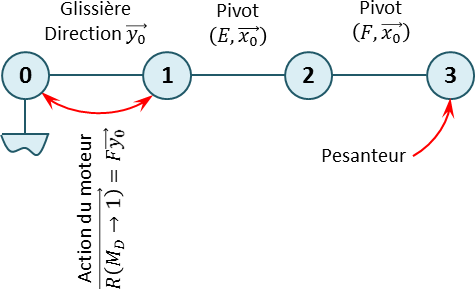
\includegraphics[width=\linewidth]{cor_01}
%\end{center}
%
%\begin{center}
%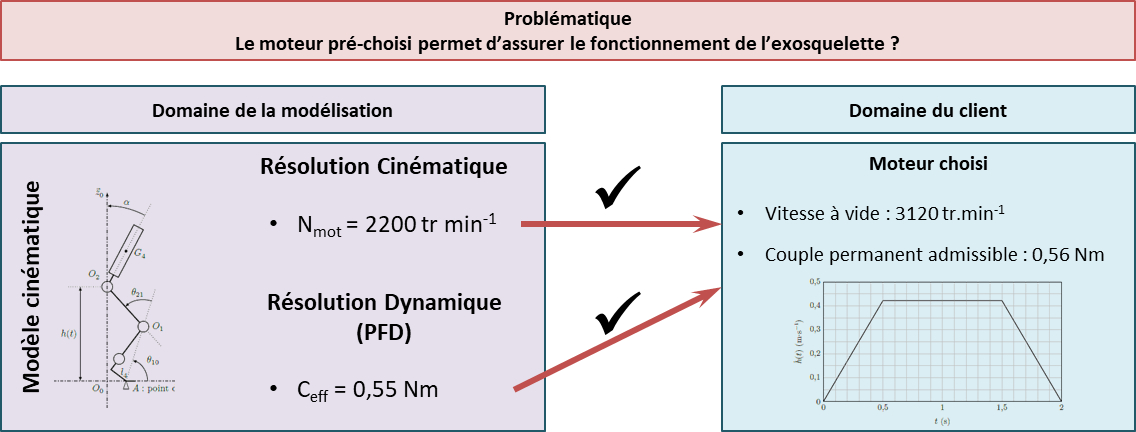
\includegraphics[width=\linewidth]{cor_02}
%\end{center}
%
%\begin{center}
%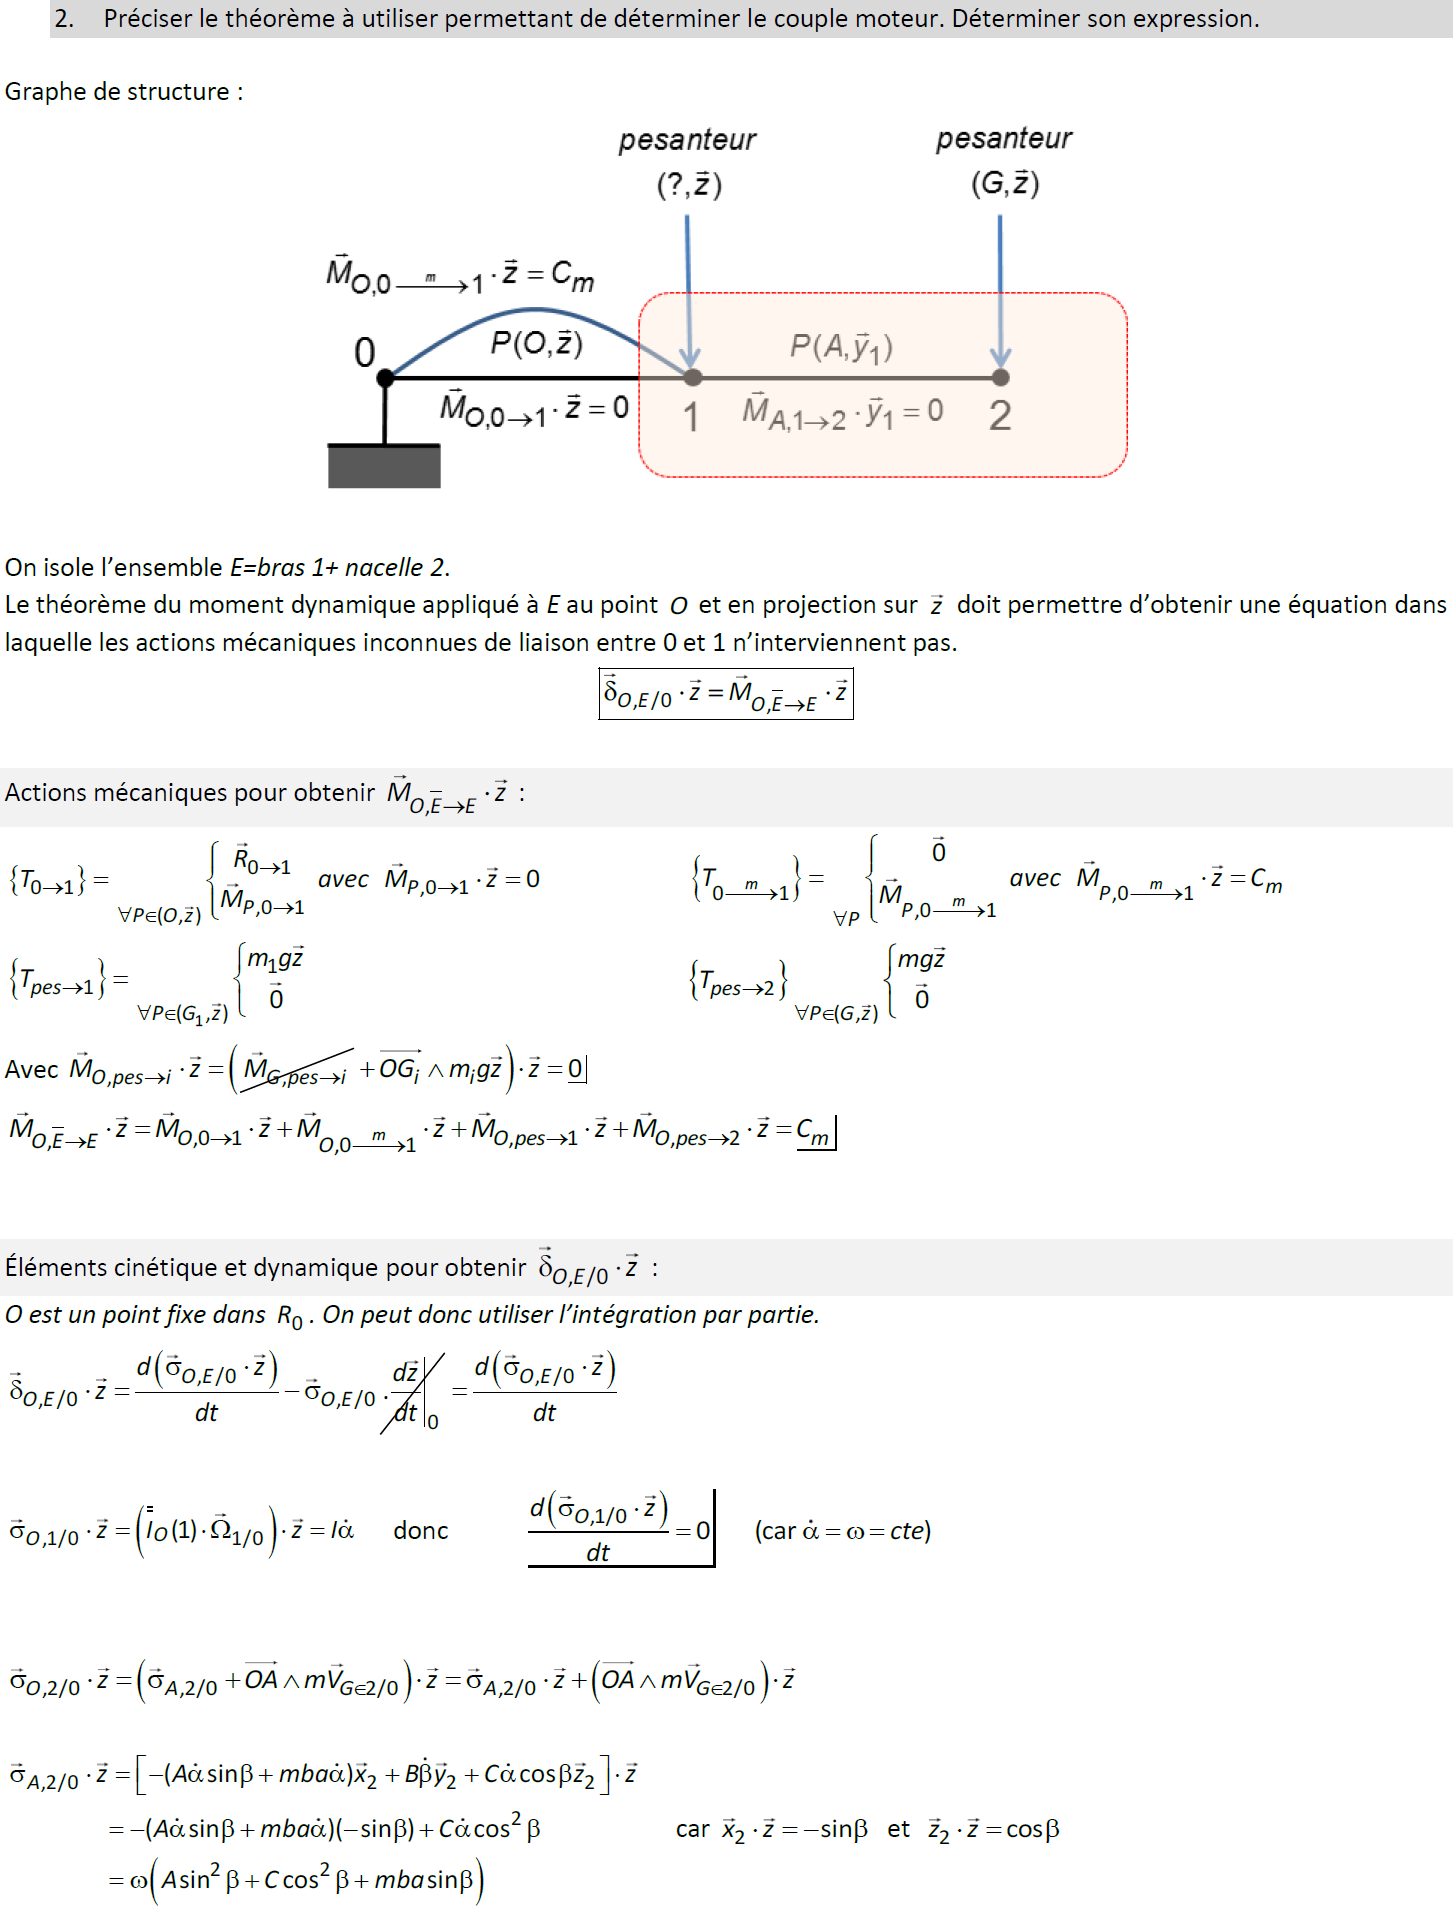
\includegraphics[width=\linewidth]{cor_03}
%\end{center}
%
%\begin{center}
%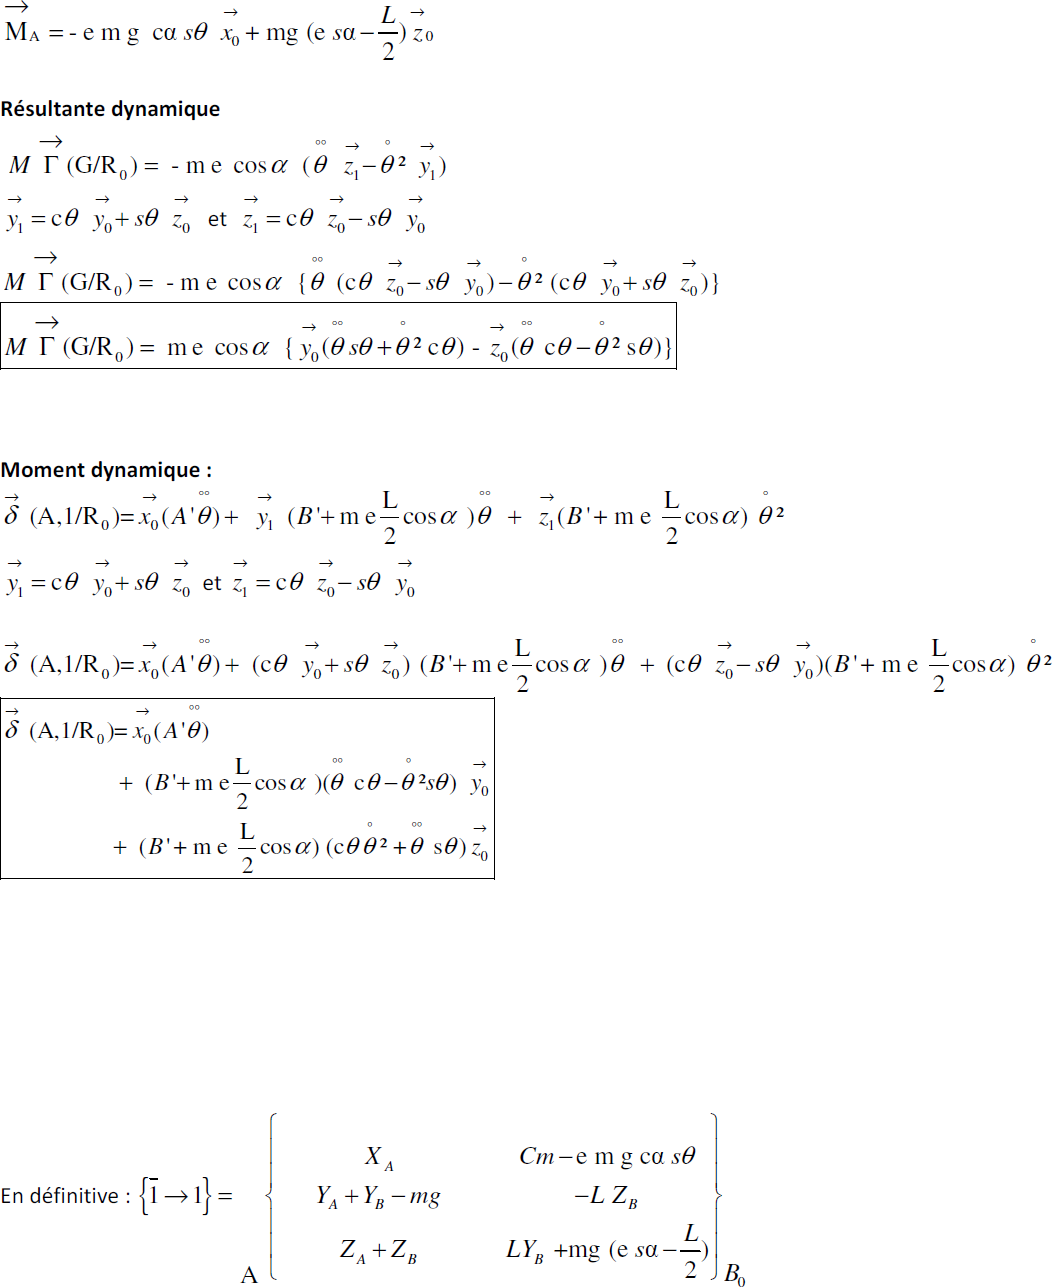
\includegraphics[width=\linewidth]{cor_04}
%\end{center}

%\begin{center}
%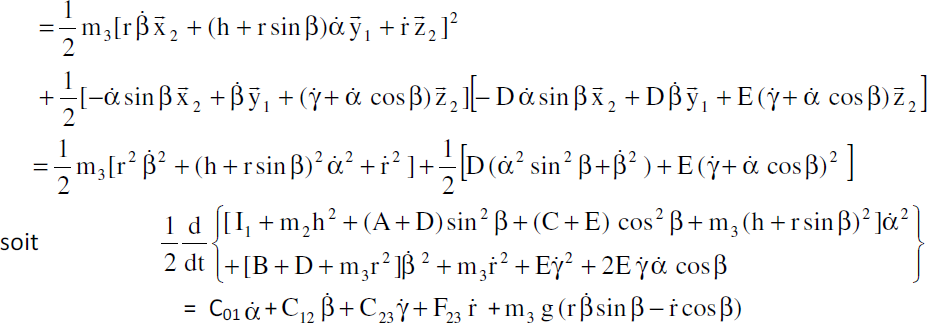
\includegraphics[width=\linewidth]{cor_05}
%\end{center}
